\documentclass{article}

\usepackage{graphicx}
\usepackage{tikz}
\usepackage{tikzsymbols}
\usetikzlibrary{calc,patterns,shapes.geometric}
\pagestyle{empty}
\usepackage[margin=0pt]{geometry}
\geometry{papersize={14in,12in}}

\def\centerarc[#1](#2)(#3:#4:#5){\draw[#1] ($(#2)+({#5*cos(#3)},{#5*sin(#3)})$) arc (#3:#4:#5);}

\begin{document}
	\begin{figure}
		\centering
		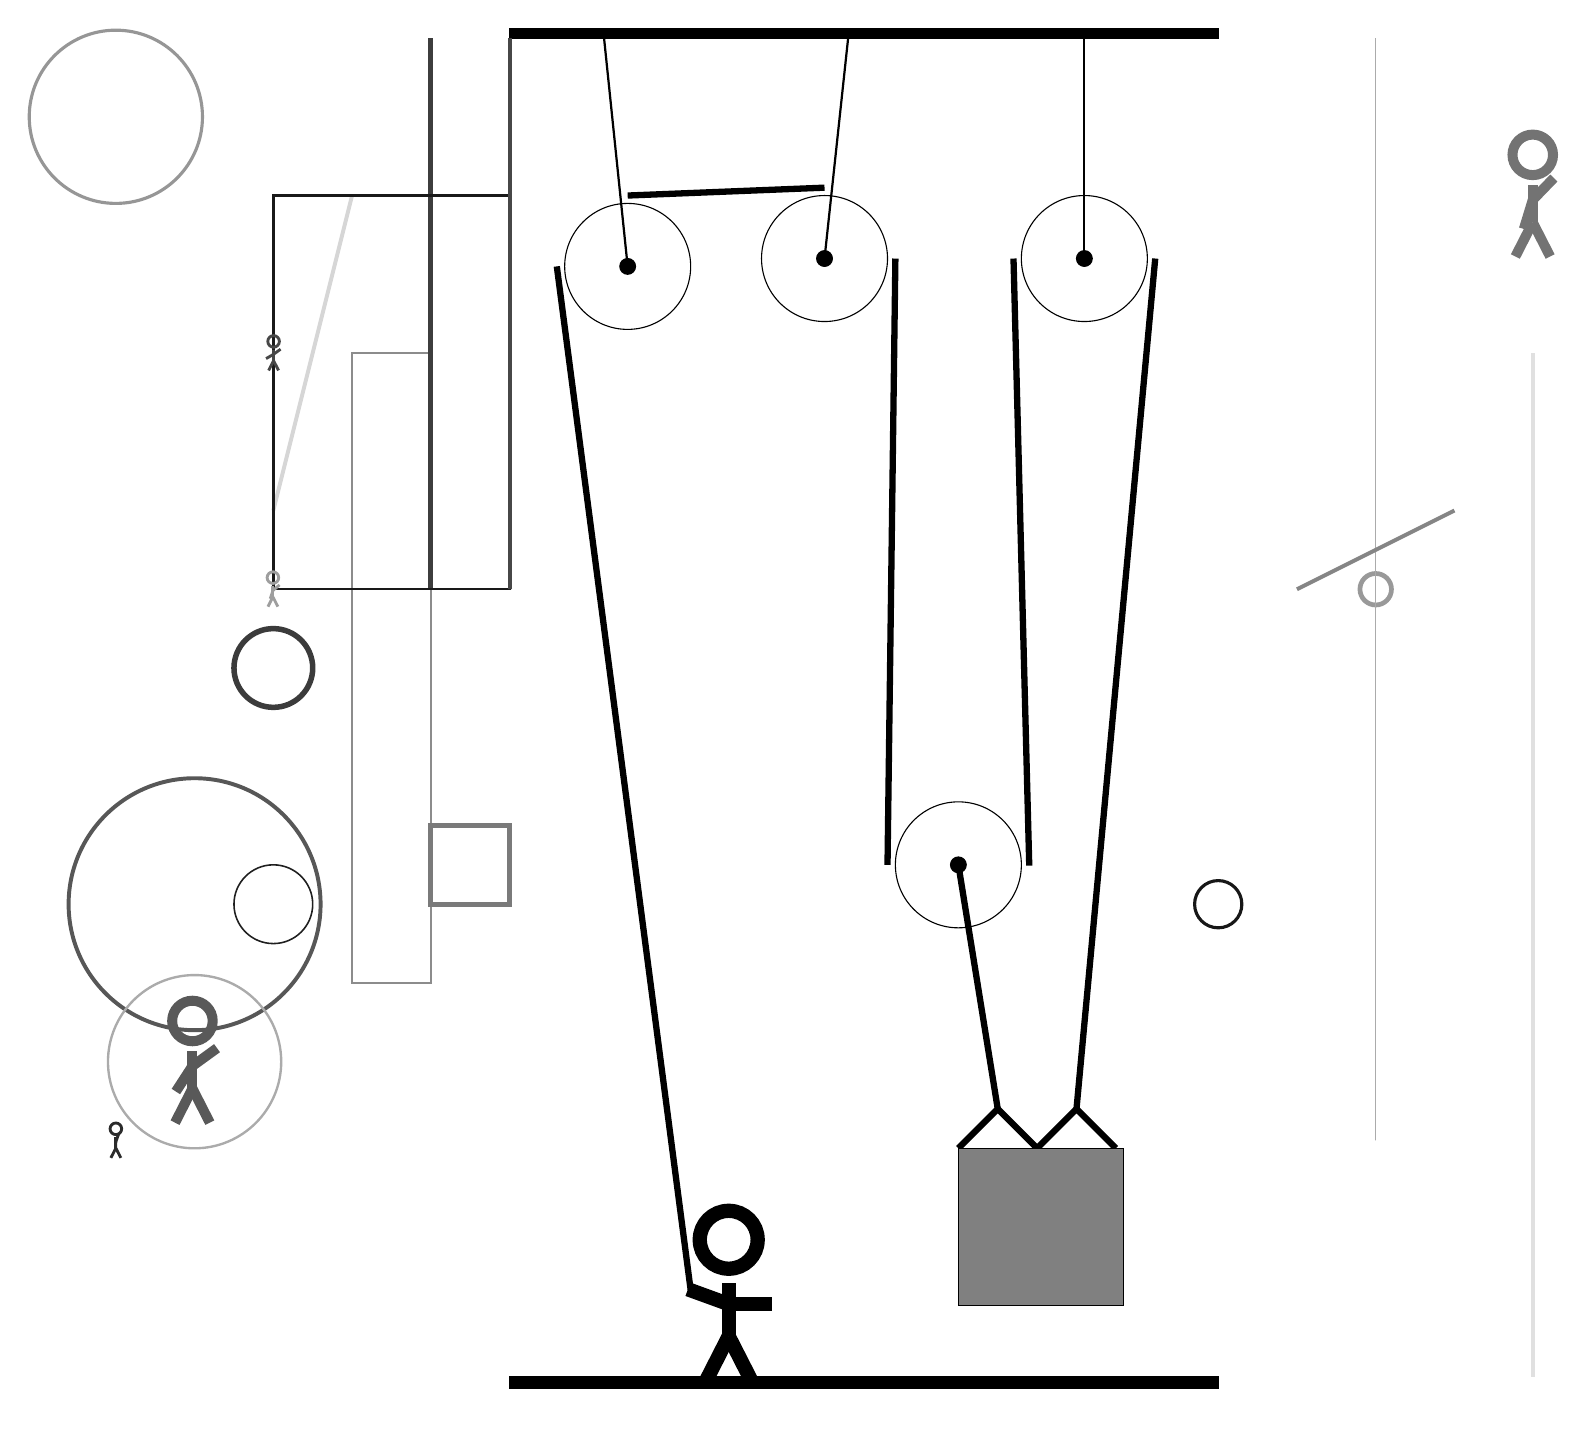
\begin{tikzpicture}
			%%%%% START %%%%%
			
			\draw[fill=black] (-3, 14) rectangle (6, 14.125);
			
			\draw (1, 11.2) circle (0.8);
			\draw[fill=black] (1, 11.2) circle (0.1);
			\draw[thick] (1, 11.2) -- (1.3, 14);
			
			\draw (4.3, 11.2) circle (0.8);
			\draw[fill=black] (4.3, 11.2) circle (0.1);
			\draw[thick] (4.3, 11.2) -- (4.3, 14);
			
			\draw (2.7, 3.5) circle (0.8);
			\draw[fill=black] (2.7, 3.5) circle (0.1);
			
			\draw[line width=0.8mm]  (2.7, -0.1) -- (3.2, 0.4) -- (3.7, -0.1) -- (4.2, 0.4) -- (4.7, -0.1);
			\draw[fill=black!50] (2.7, -0.1) rectangle (4.8, -2.1);
			
			\draw (-1.5, 11.1) circle (0.8);
			\draw[fill=black] (-1.5, 11.1) circle (0.1);
			\draw[thick] (-1.5, 11.1) -- (-1.8, 14);
			
			\draw[line width=0.2mm, color=black!45] (-5, 2) rectangle (-4, 10);
			
			\draw [line width=0.6mm, color=black!40](8, 7) circle (0.2);
			\draw[line width=0.2mm, color=black!33] (8, 14) rectangle (8, 0);
			\draw[line width=0.5mm, color=black!16](-5, 12) -- (-6, 8);
			\draw[line width=0.5mm, color=black!48](9, 8) -- (7, 7);
			\node[line width=0.3mm, color=black!83] at (-8, 0) {\Strichmaxerl[2][87][70]};
			\draw[line width=0.6mm, color=black!76] (-4, 14) rectangle (-4, 7);
			
			\draw[line width=0.6mm, color=black!52] (-3, 3) rectangle (-4, 4);
			\draw[line width=0.3mm, color=black!90] (-3, 7) rectangle (-6, 12);
			\draw [line width=0.5mm, color=black!66](-7, 3) circle (1.6);
			
			\draw[line width=0.5mm, color=black!72] (-3, 7) rectangle (-3, 14);
			
			\node[line width=0.5mm, color=black!72] at (-6, 10) {\Strichmaxerl[2][30][36]};
			\draw [line width=0.2mm, color=black!88](-6, 3) circle (0.5);
			
			\draw [line width=0.4mm, color=black!41](-8, 13) circle (1.1);
			\draw [line width=0.7mm, color=black!77](-6, 6) circle (0.5);
			\node[line width=0.2mm, color=black!65] at (-7, 1) {\Strichmaxerl[7][57][36]};
			
			\node[line width=0.7mm, color=black!38] at (-6, 7) {\Strichmaxerl[2][72][40]};
			
			\draw[line width=0.5mm, color=black!12](10, 10) -- (10, -3);
			\draw [line width=0.3mm, color=black!33](-7, 1) circle (1.1);
			\node[line width=0.6mm, color=black!55] at (10, 12) {\Strichmaxerl[7][73][46]};
			\draw [line width=0.4mm, color=black!91](6, 3) circle (0.3);
			
			
			\draw[line width=0.8mm](-0.7, -1.9) --  (-2.4, 11.1);
			\centerarc[line width=0.8mm](-1.5, 11.1)(90:180:0.9);
			\draw[line width=0.8mm](-1.5, 12.0) -- (1, 12.1);
			\centerarc[line width=0.8mm](1, 11.2)(0:90:0.9);
			\draw[line width=0.8mm](1.9, 11.2) -- (1.8, 3.5);
			\centerarc[line width=0.8mm](2.7, 3.5)(180:370:0.9);
			\draw[line width=0.8mm] (3.6, 3.49) -- (3.4, 11.2);
			\centerarc[line width=0.8mm](4.3, 11.2)(0:180:0.9);
			\draw[line width=0.8mm](4.2, 0.4) -- (5.2, 11.2);
			\draw[line width=0.8mm] (3.2, 0.4) -- (2.7, 3.5);
			
			\node at (-0.2, -2) {\Strichmaxerl[10][-20][0]};
			
			\draw[fill=black] (-3, -3) rectangle (6, -3.15);
			
			%%%%% END %%%%%
		\end{tikzpicture}
	\end{figure}	
\end{document}